
\section{Noms vernaculaires et noms scientifiques correspondants}
 
 Liste alphabétique des noms vulgaires ou des noms vernaculaires attestés8 en français.
Note : certaines espèces ont plusieurs noms. L'abréviation « spp. » veut dire « les espèces »
Les classifications évoluant encore, certains noms scientifiques ont peut-être un autre synonyme valide.

\begin{multicols}{2}
    \begin{itemize}
  
\item Grenouille agile - Rana dalmatina \up{9,5}
\item Grenouille d'Albanie - Pelophylax shqipericus \up{9}
\item Grenouille arboricole - Hylidae spp. et Rhacophoridae spp.
\item Grenouille arboricole d'Afrique - Leptopelis modestus \up{5}
\item Grenouille des Balkans - Pelophylax kurtmuelleri \up{9}
\item Grenouille de Berger - Rana bergeri \up{9}
\item Grenouille des bois - Rana sylvatica \up{9}
\item Grenouille des champs - Rana arvalis \up{9,5}
\item Grenouille des montagnes à pattes jaunes - Rana muscosa
\item Grenouille du ciel - Rhacophorus omeimontis \up{5}
\item Grenouille maculée de Columbia - Rana luteiventris \up{10}
\item Grenouille maculée de l'Orégon - Rana pretiosa \up{10}
\item Grenouille marsupiale - Gastrotheca spp \up{5}
\item Grenouille-mouton - Hypopachus cuneus \up{5}
\item Grenouille mugissante - Rana catesbeiana
\item Grenouille du Nord - Rana septentrionalis \up{9}
\item Grenouille oxyrhine - Rana arvalis
\item Grenouille de Pérez - Pelophylax perezi \up{5}
\item Grenouille pisseuse - Rana dalmatina
\item Grenouille des Pyrénées - Rana pyrenaica \up{9}
\item Grenouille-à-queue côtière - Ascaphus truei \up{10}
\item Grenouille-à-queue des Rocheuses - Ascaphus montanus \up{10}
\item Grenouille rieuse - Pelophylax ridibundus \up{9,5}
\item Grenouille rousse - Rana temporaria \up{9,5}
\end{itemize}
\end{multicols}    

\begin{figure}
 \begin{center}
 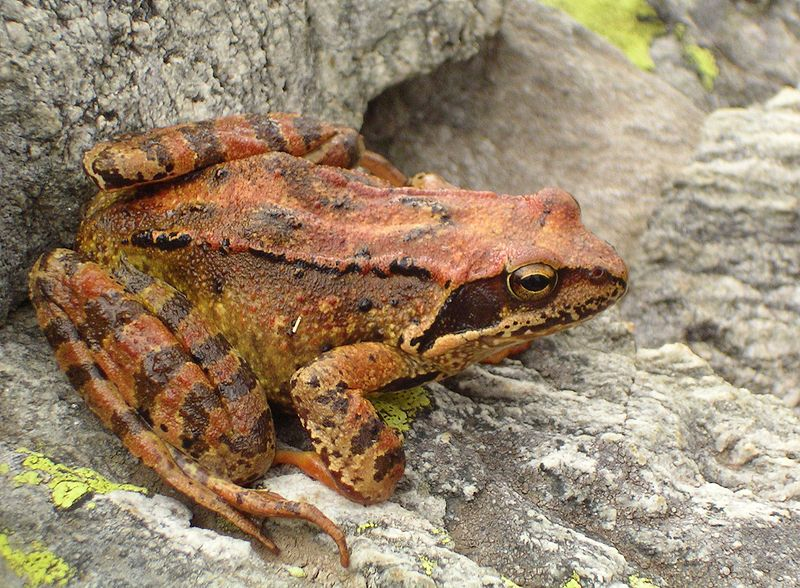
\includegraphics[scale=0.3]{Grenouille_rousse.jpg}
 \caption{Grenouille rousse}
 \end{center}
\end{figure}
 
\begin{figure}
 \begin{center}
  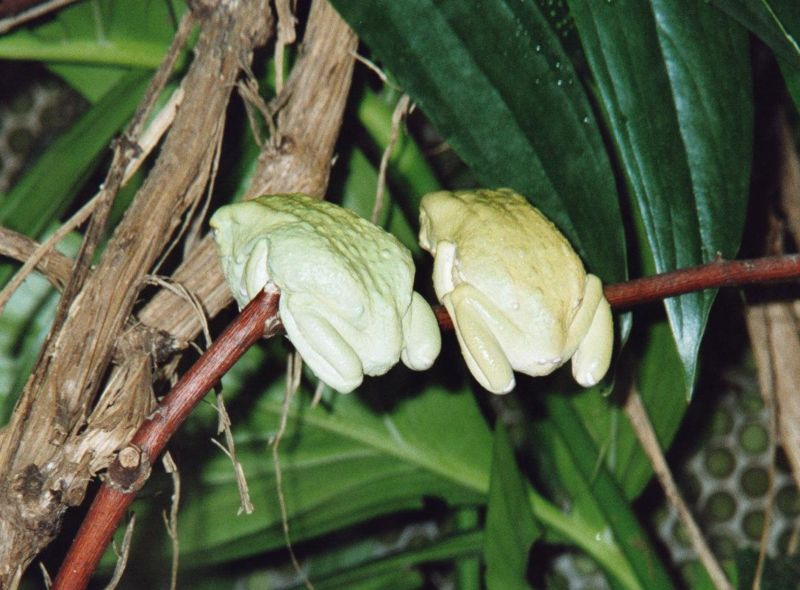
\includegraphics[scale=0.3]{grenouille_volante.jpg}
  \caption{Grenouille volante}
 \end{center}
\end{figure}

    
    

